% gm-termtest-C-mock.tex

\documentclass[11pt]{article}
\usepackage{enumerate}
\usepackage{syllogism} 
\usepackage{october}
\usepackage[table]{xcolor}

\begin{document}

\textbf{Term Test C Exercises and Instructions}

There will be four questions on term test C, in two parts.

\begin{enumerate}
\item (Part I)
  \begin{enumerate}
  \item Identify the features of two conic sections.
  \item Simplify two expressions, for which you may want to use
    factoring. These questions may come in the form of an equation.
  \end{enumerate}
\item (Part II)
  \begin{enumerate}
  \item Two word problems, one for solving triangles and one for
    logarithms and exponents (exponential growth/decay).
  \item Three equations, a trigonometric equation, an exponential
    equation, and a logarithmic equation.
  \end{enumerate}
\end{enumerate}

1. Identify the required features of the following conic sections
(parabola: vertex; ellipse: centre and dimensions; circle: centre and
radius; hyperbola: centre, dimensions, asymptotes). Draw a diagram.

% 8
\begin{equation}
  \label{eq:ohdiedoe}
4x^{2}-9y^{2}-8x-198y=1049
\end{equation}

% 6
\begin{equation}
  \label{eq:mahbeizo}
4y^{2}+80y+384=-x^{2}
\end{equation}

% 4
\begin{equation}
  \label{eq:ohwoojie}
16x(x+1)+8y(2y+3)=131
\end{equation}

% 7
\begin{equation}
  \label{eq:chohtohk}
x^{2}-y^{2}+4x+6y=6
\end{equation}

% 2
\begin{equation}
  \label{eq:gofushoo}
y(y-4)-x=2
\end{equation}

% 1
\begin{equation}
  \label{eq:vibeibie}
3x^{2}+\sqrt{252}x-y+23=0
\end{equation}

% 3
\begin{equation}
  \label{eq:aepheipi}
x^{2}+y^{2}-8x+6y=(\pi-5)(\pi+5)
\end{equation}

% 5
\begin{equation}
  \label{eq:vogeobab}
x^{2}+4y^{2}-2x+24y+33=0
\end{equation}

2a. Solve the following equations for positive values less than
$360^{\circ}$. 
% Welchons Krickenberger page 216f
\begin{equation}
  \label{eq:uxohjeib}
\sin{}2x=2\sin{}x
\end{equation}
\begin{equation}
  \label{eq:eicohrae}
\sin{}2x+2\cos{}2x=1
\end{equation}
\begin{equation}
  \label{eq:epuufeca}
\sin{}2x=\cos{}x
\end{equation}
\begin{equation}
  \label{eq:weungodu}
\sin{}2y=\tan{}y
\end{equation}
\begin{equation}
  \label{eq:oraighah}
\sin{}3z+\sin{}z=0
\end{equation}
\begin{equation}
  \label{eq:saenonge}
\cos{}x=\sin\frac{x}{2}
\end{equation}
\begin{equation}
  \label{eq:eeghoghi}
\tan{}2w=\cot{}w
\end{equation}
\begin{equation}
  \label{eq:eesicaet}
\tan{}2x=2\sin{}x
\end{equation}
\begin{equation}
  \label{eq:fixahfee}
2\sin^{2}\frac{1}{2}y-\cos{}y=2
\end{equation}
\begin{equation}
  \label{eq:iesiwoox}
\sin^{2}x=1-\sin{}2x
\end{equation}
\begin{equation}
  \label{eq:eemengaj}
  \cos{}4x+\cos{}2x=0
\end{equation}

2b. Solve the following exponential and logarithmic equations
(solutions are in D2L in the module for lesson 12).
% lecture notes
\begin{equation}
  \label{eq:faeyeije}
  3^{x+2}=7
\end{equation}
\begin{equation}
  \label{eq:ochedoxi}
  8e^{2x}=20
\end{equation}
\begin{equation}
  \label{eq:veipoeyu}
  e^{3-2x}=4
\end{equation}
\begin{equation}
  \label{eq:aquusahm}
  3x^{2}e^{x}+x^{3}e^{x}=0
\end{equation}
  \begin{equation}
    \label{eq:rohkiine}
    4^{1-2x}=2
  \end{equation}
  \begin{equation}
    \label{eq:zahsuini}
    8^{6+3x}=4
  \end{equation}
  \begin{equation}
    \label{eq:iaphaeya}
    3^{x^{2}+x}=\sqrt{3}
  \end{equation}
  \begin{equation}
    \label{eq:iebaiviu}
    4^{x-x^{2}}=\frac{1}{2}
  \end{equation}
  \begin{equation}
    \label{eq:maareiju}
    \log_{x}64=-3
  \end{equation}
  \begin{equation}
    \label{eq:sheuroov}
    \log_{\sqrt{2}}x=-6
  \end{equation}
  \begin{equation}
    \label{eq:dairithe}
    5^{x}=3^{x+2}
  \end{equation}
  \begin{equation}
    \label{eq:seizieng}
    5^{x+2}=7^{x-2}
  \end{equation}
  \begin{equation}
    \label{eq:ceivapuw}
    9^{2x}=27^{3x-4}
  \end{equation}
  \begin{equation}
    \label{eq:eefohvoh}
    25^{2x}=5^{x^{2}-12}
  \end{equation}
  \begin{equation}
    \label{eq:xiefepib}
    \log_{3}\sqrt{x-2}=2
  \end{equation}
  \begin{equation}
    \label{eq:eegaifah}
    2^{x+1}\cdot{}8^{-x}=4
  \end{equation}
  \begin{equation}
    \label{eq:phahmobu}
    8=4^{x^{2}}\cdot{}2^{5x}
  \end{equation}
  \begin{equation}
    \label{eq:xonguoge}
    2^{x}\cdot{}5=10^{x}
  \end{equation}
  \begin{equation}
    \label{eq:aeshaite}
    \log_{6}(x+3)+\log_{6}(x+4)=1
  \end{equation}
  \begin{equation}
    \label{eq:eequabae}
    \log(7x-12)=2\log{}x
  \end{equation}
  \begin{equation}
    \label{eq:niephait}
    e^{1-x}=5
  \end{equation}
  \begin{equation}
    \label{eq:eophooki}
    e^{1-2x}=4
  \end{equation}
  \begin{equation}
    \label{eq:eevaicei}
    2^{3x}=3^{2x+1}
  \end{equation}
  \begin{equation}
    \label{eq:ohquaiva}
    2^{x^{3}}=3^{x^{2}}
  \end{equation}
  \begin{equation}
    \label{eq:poikeeng}
    2^{\frac{2}{\log_{5}x}}=\frac{1}{16}
  \end{equation}
\begin{equation}
  \label{eq:haesiiro}
  e^{2x}-e^{x}-6=0
\end{equation}

3. Simplify the following expressions.
% James Stewart, page 42
\begin{equation}
  \label{eq:ceedarai}
\frac{2x^{3}-x^{2}-6x}{2x^{2}-7x+6}
\end{equation}
\begin{equation}
  \label{eq:ohchahph}
\frac{1-x^{2}}{x^{2}-1}
\end{equation}
\begin{equation}
  \label{eq:eiwaegeb}
\frac{x^{2}-x-6}{x^{2}+2x}\cdot\frac{x^{3}+x^{2}}{x^{2}-2x-3}
\end{equation}
\begin{equation}
  \label{eq:eithuogh}
\frac{\frac{x^{3}}{x+1}}{\frac{x}{x^{2}+2x+1}}
\end{equation}
\begin{equation}
  \label{eq:aehohthu}
\frac{1}{x+1}+\frac{1}{x-1}
\end{equation}
\begin{equation}
  \label{eq:iewugeth}
\frac{5}{2x-3}-\frac{3}{(2x-3)^{2}}
\end{equation}
\begin{equation}
  \label{eq:tiphaike}
1+\frac{1}{1+\frac{1}{1+x}}
\end{equation}
\begin{equation}
  \label{eq:guoquoht}
\frac{x}{x^{2}+x-2}-\frac{2}{x^{2}-5x+4}
\end{equation}
\begin{equation}
  \label{eq:moogahve}
\sqrt{1+\left(x^{3}-\frac{1}{4x^{3}}\right)^{2}}
\end{equation}

4. Solve the following word problems.

a. What rate of inflation doubles prices every 14 years? Use the
formula for compound interest:
\begin{equation}
  \label{eq:quahphia}
    A=P\left(1+\frac{r}{m}\right)^{mt}
\end{equation}
\begin{tabular}{rcl}
  $A$&\ldots&accumulated amount at the end of $t$ years \\
  $P$&\ldots&principal \\
  $r$&\ldots&interest rate p.a. \\
  $m$&\ldots&number of conversion periods per year \\
  $t$&\ldots&term (number of years)
\end{tabular}

b. Here is Newton's Law of Cooling:
\begin{equation}
  \label{eq:iemahbec}
  u(t)=T+(u(0)-T)e^{kt}
\end{equation}
The hotel Bora-Bora is having a pig roast. At noon, the chef put the
pig in a large earthen oven. The pig's original temperature was
$75^{\circ}F$. At 2:00\textsc{pm} the chef checked the pig's
temperature and was upset because it had reached only $100^{\circ}F$.
If the oven's temperature remains a constant $325^{\circ}F$, at what
time may the hotel serve its guests, assuming that pork is done when
it reaches $175^{\circ}F$?

For (c) and (d), the formula for uninhibited exponential growth is
\begin{equation}
  \label{eq:xufuacoo}
  A(t)=A(0)e^{kt}
\end{equation}

c. A culture starts with 8600 bacteria. After one hour the count is
$10,000$. (i) Find the number of bacteria after 2 hours. (ii) After
how many hours will the number of bacteria double?

d. The number of people living in a country is increasing each year
exponentially. The number of people 5 years ago was 4 million. The
number of people in five years is projected to be 6.25 million. What
is the present population of the country?

\newpage

e. The robot arm shown in the figure places packages on a conveyor
belt. What is the distance $x$?

\begin{figure}[h]
   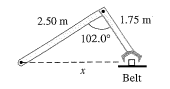
\includegraphics[scale=.5]{./tri-01.png}
\end{figure}

f. Find the angle between the front legs and the back legs of the
folding chair shown in the figure.

\begin{figure}[h]
   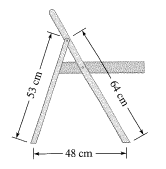
\includegraphics[scale=.5]{./tri-02.png}
\end{figure}

g. A damper mechanism in an air-conditioning system is shown. If
$\theta=27.5^{\circ}$ when the spring is at its shortest and
longest lengths, what are these lengths?

\begin{figure}[h]
   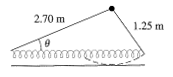
\includegraphics[scale=.5]{./tri-10.png}
\end{figure}

\end{document}

